\section{Studies of signal and background separation using calorimeter clusters}
%%In the future detector, when the energy is increased, the boost jet is bigger, and it will be more difficult to distinguish the signal and the background. In this section, we want to study different variables and see their ability to separate the signal and the background in different detector sizes in the clustering of detector-level.\\
In this section, we study different jet substructure variables and compare their ability to separate the signal and the background for different detector sizes using calorimeter clusters.\\
%%Figure 3 to 5 show the ROC curves of three variables, $c2b1$ , $\tau_{21}$, and $\tau_{32}$. For each variable, there are three different sizes of the sub-detector HCAL compared at four special collision energies. For different sizes, the one with the highest background rejection rate, which is 1-background efficiency, at the same signal efficiency has the best separate ability.

Figures 3--5 show the ROC curves of three variables, $c_2^{(1)}$~\cite{Larkoski:2013eya} , $\tau_{21}$~\cite{Thaler:2010tr}, and $\tau_{32}$~\cite{Thaler:2010tr}, respectively. Three different cell sizes of the HCAL are compared for four collision energies. For different cell sizes with the same signal efficiency, the one with the highest background rejection rate, namely (1-background efficiency), has the highest separate power.\\

In Figure 3 for the variable $c_2^{(1)}$ , the ROC curves of the three detector cell sizes are close to each other for each collision energy. Therefore, this variable is not sensitive to the detector cell size.\\

For the $\tau_{21}$ variable in Figure 4, at 5 TeV, the smallest detector size (1$\times$1 cm) can separate the background from the signal well. However, this is not the usual case as the ROC curves nearly merge together at higher collision energy. In addition, the detector with the bigger size tends to have higher separation power than the smaller detector size in 20 and 40 TeV collision energy.\\

Figure 5 shows the variable $\tau_{32}$, where the smallest detector size has the best separation power for all collision energies.\\

In conclusion, in all the cases of energy and detector size, the variable $c_2^{(1)}$ has the best separation power compared to the other two variables. In addition, the variable $\tau_{32}$ follows the expectation that smaller detector size has better separation power.\\

\label{sec:efficiency}


\begin{figure}
\begin{center}
   \subfigure[5 TeV] {
   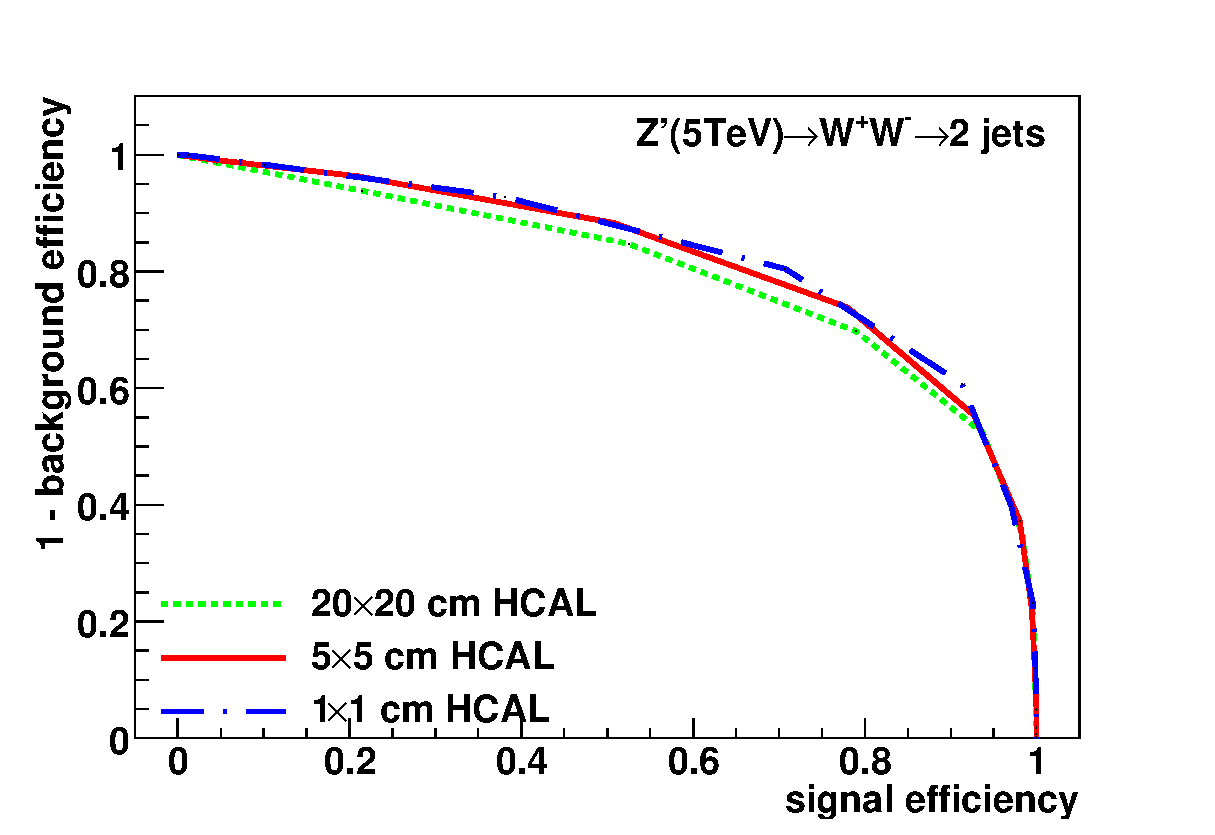
\includegraphics[width=0.43\textwidth]{figs/cluster_c2b1_5_tev_eff.eps}\hfill
   }
   \subfigure[10 TeV] {
   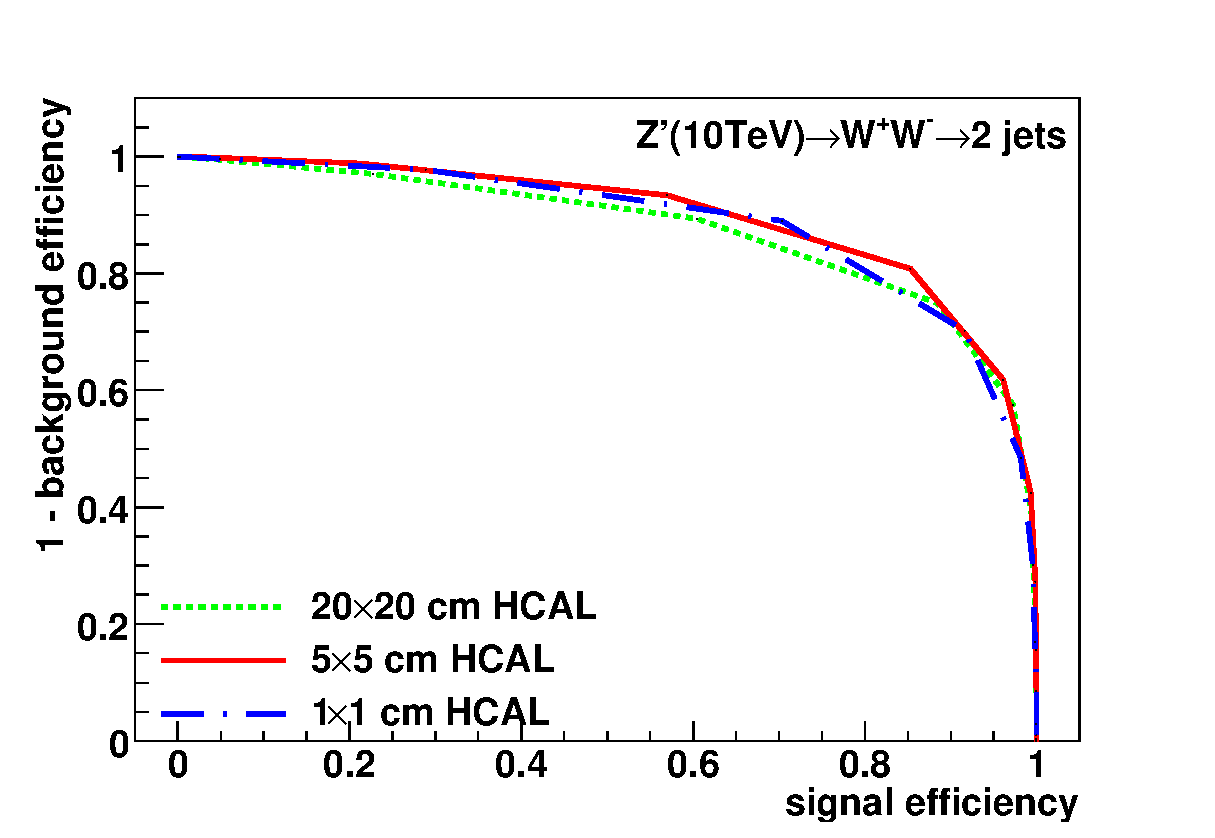
\includegraphics[width=0.43\textwidth]{figs/cluster_c2b1_10_tev_eff.eps}
   }
   \subfigure[20 TeV] {
   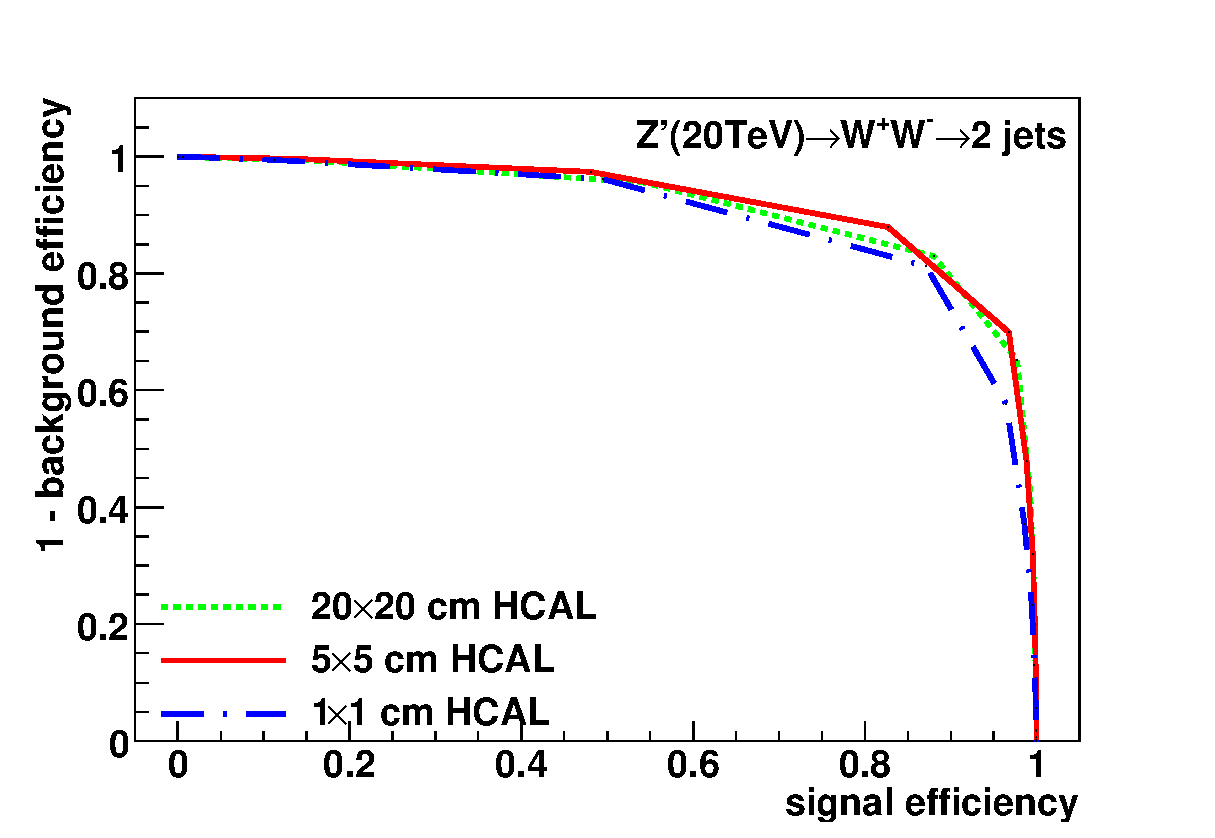
\includegraphics[width=0.43\textwidth]{figs/cluster_c2b1_20_tev_eff.eps}
   }
   \subfigure[40 TeV] {
   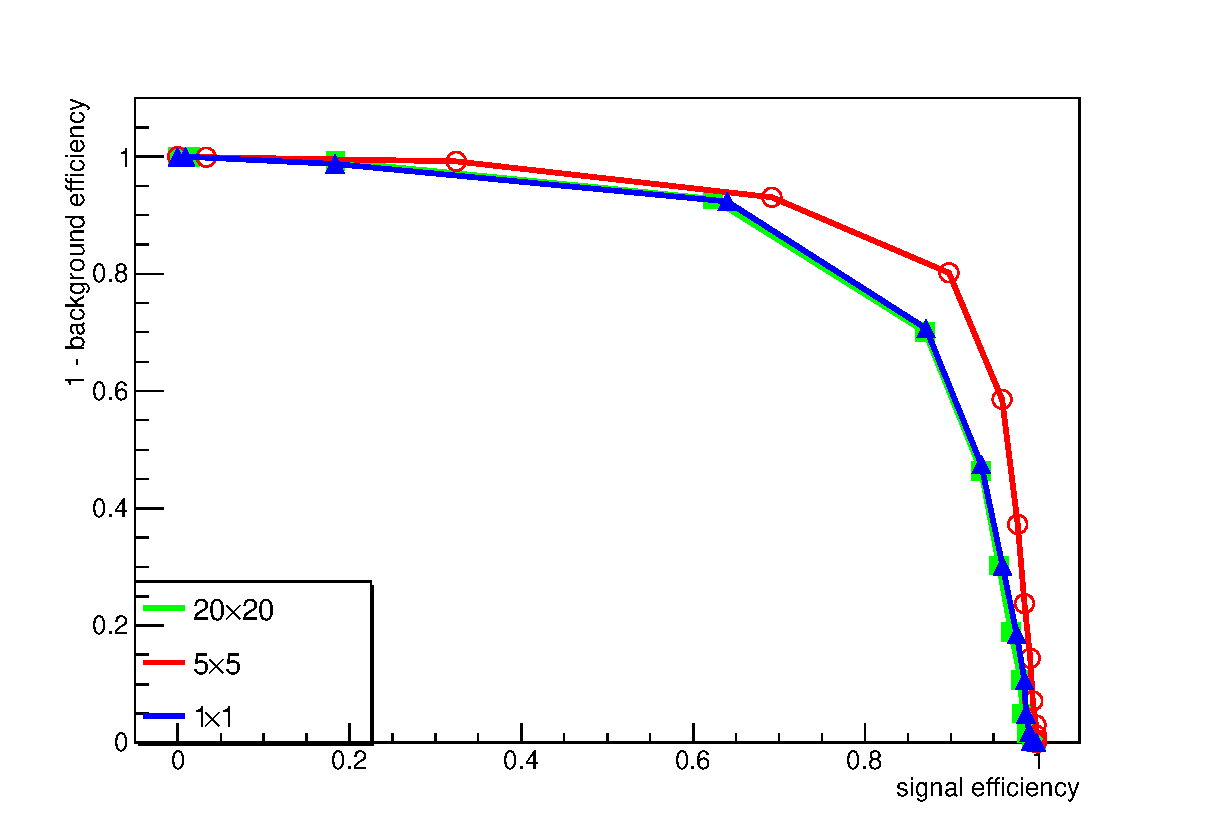
\includegraphics[width=0.43\textwidth]{figs/cluster_c2b1_40_tev_eff.eps}
   }
\end{center}
\caption{Signal efficiency versus background rejection rate using $c_2^{(1)}$.The energies of collision at (a)5, (b)10, (c)20, (d)40TeV are shown here. In each picture, the three ROC curves correspond to different detector sizes.}
\label{fig:cluster_c2b1}
\end{figure}


\begin{figure}
\begin{center}
   \subfigure[5 TeV] {
   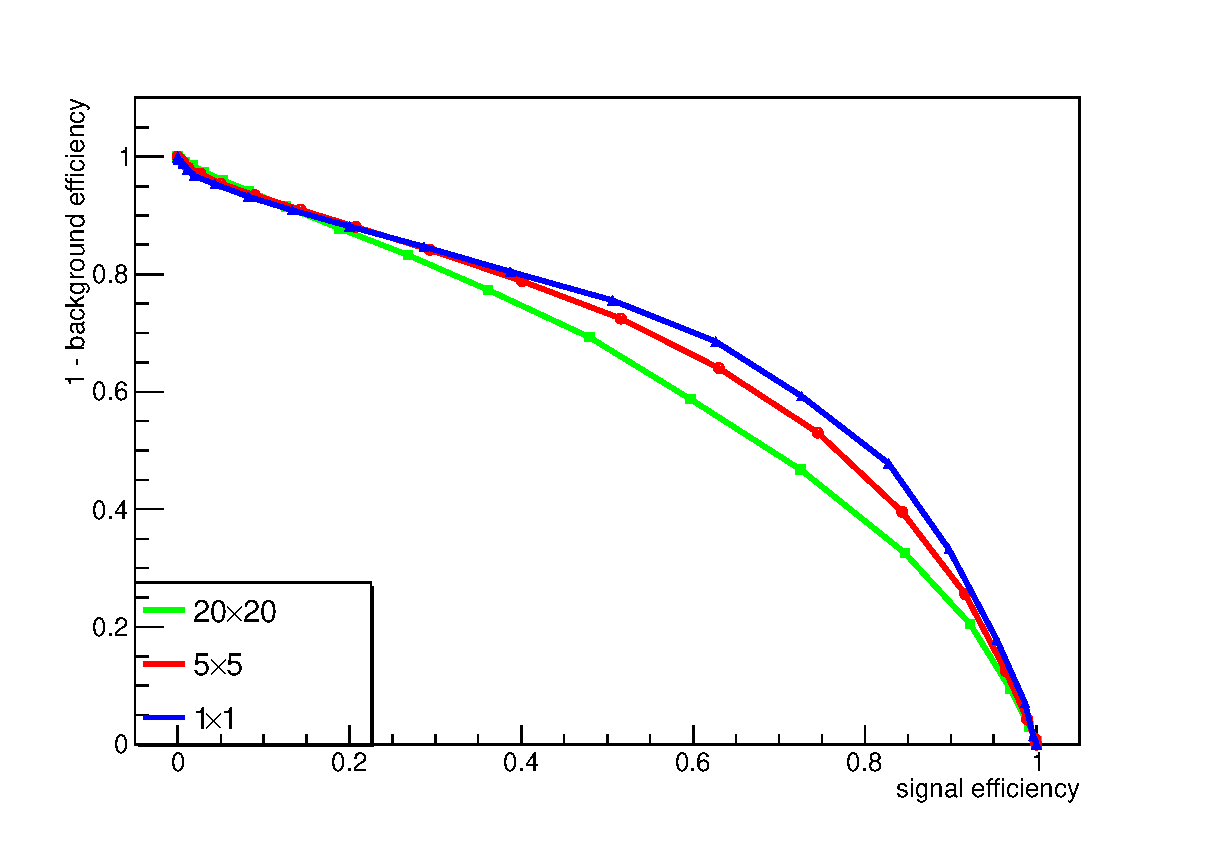
\includegraphics[width=0.43\textwidth]{figs/cluster_tau21_5_tev_eff.eps}\hfill
   }
   \subfigure[10 TeV] {
   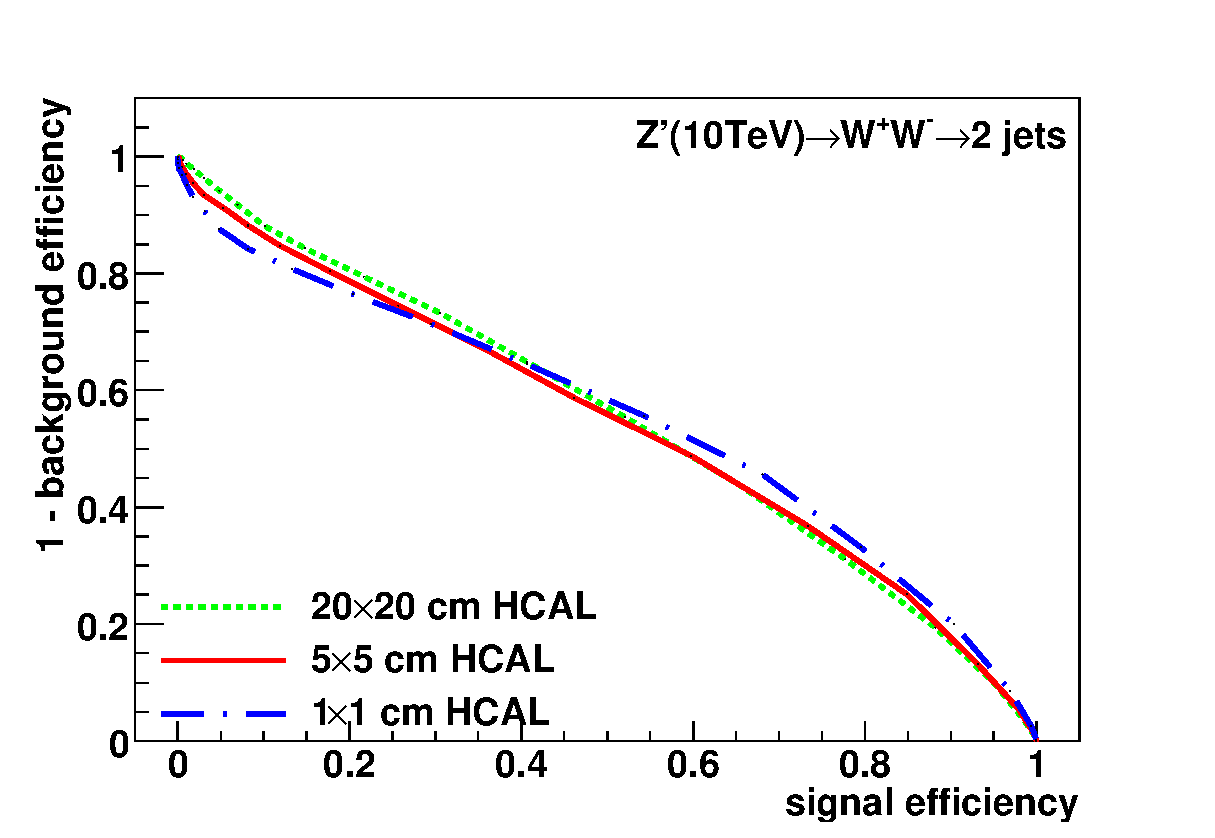
\includegraphics[width=0.43\textwidth]{figs/cluster_tau21_10_tev_eff.eps}
   }
   \subfigure[20 TeV] {
   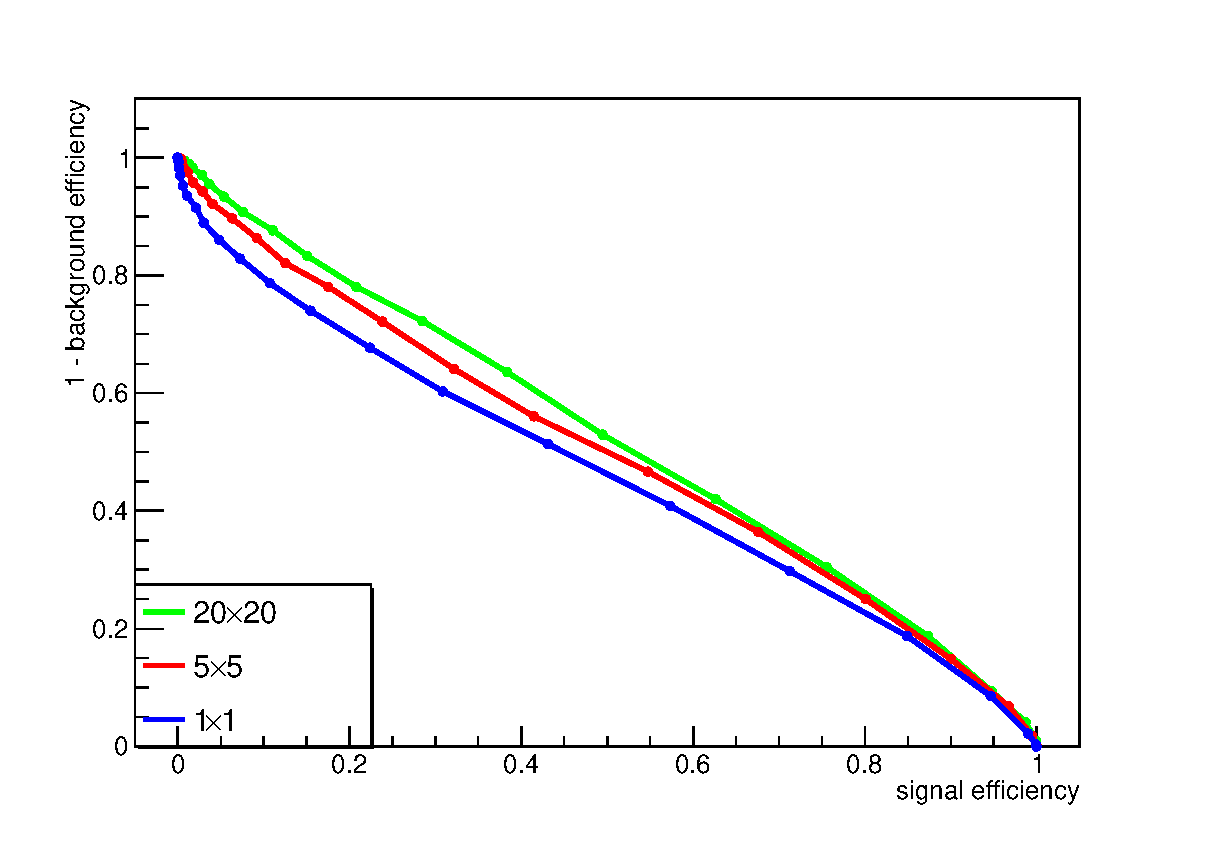
\includegraphics[width=0.43\textwidth]{figs/cluster_tau21_20_tev_eff.eps}
   }
   \subfigure[40 TeV] {
   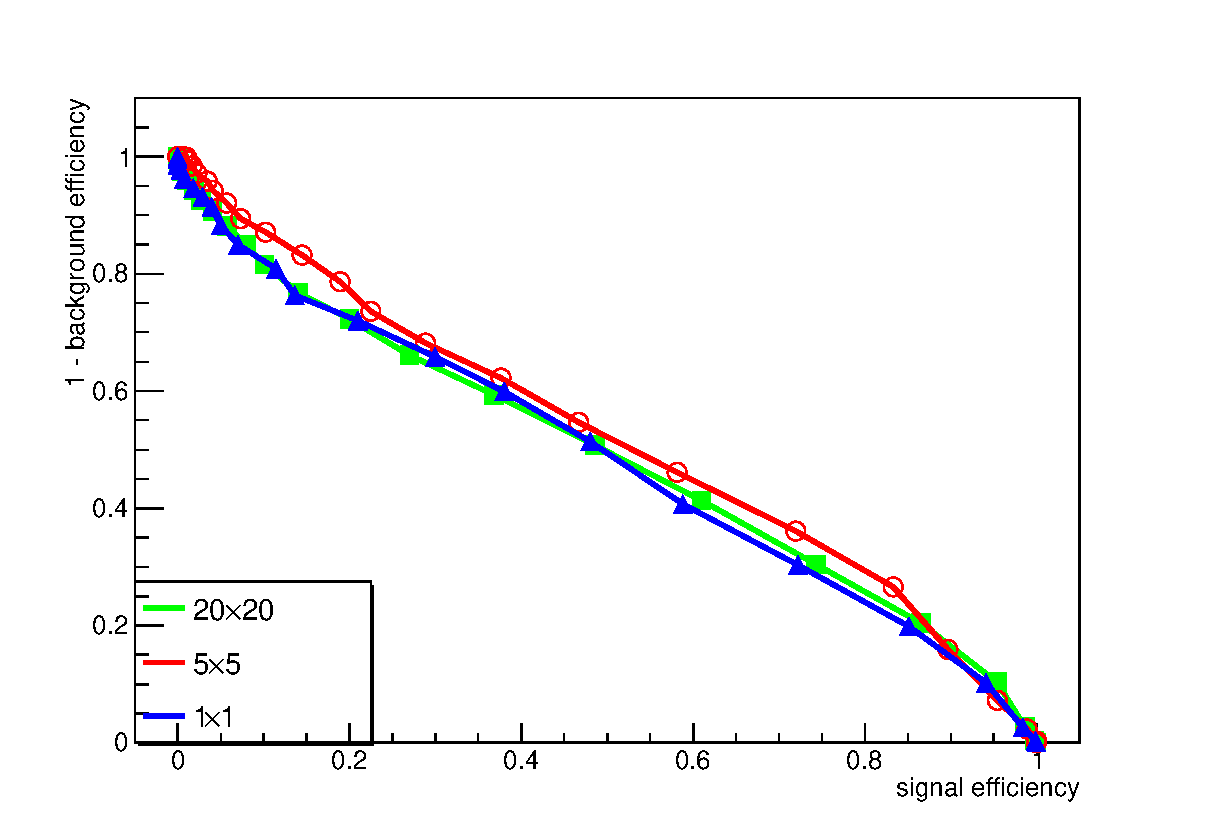
\includegraphics[width=0.43\textwidth]{figs/cluster_tau21_40_tev_eff.eps}
   }
\end{center}
\caption{Signal efficiency versus background rejection rate using $\tau_{21}$.The energies of collision at (a)5, (b)10, (c)20, (d)40TeV are shown here. In each picture, the three ROC curves correspond to different detector sizes.}
\label{fig:cluster_tau21}
\end{figure}


\begin{figure}
\begin{center}
   \subfigure[5 TeV] {
   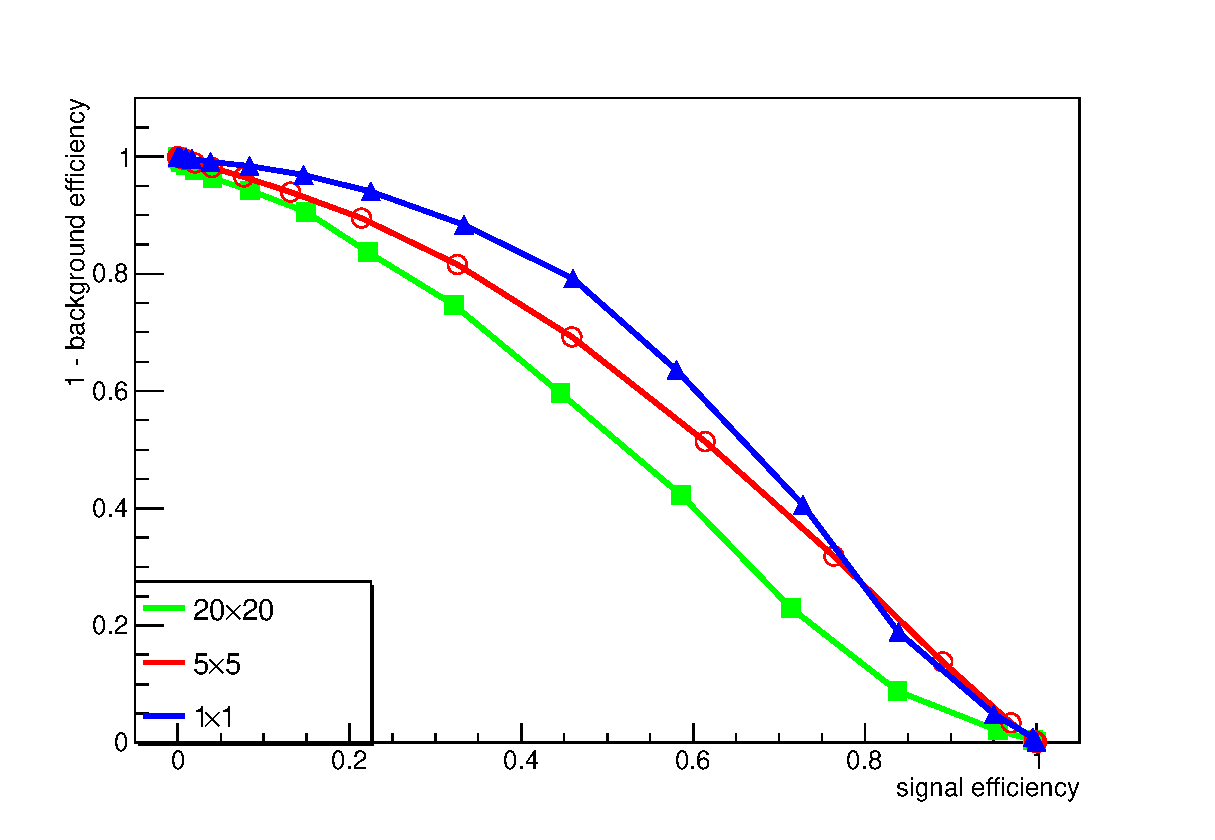
\includegraphics[width=0.43\textwidth]{figs/cluster_tau32_5_tev_eff.eps}\hfill
   }
   \subfigure[10 TeV] {
   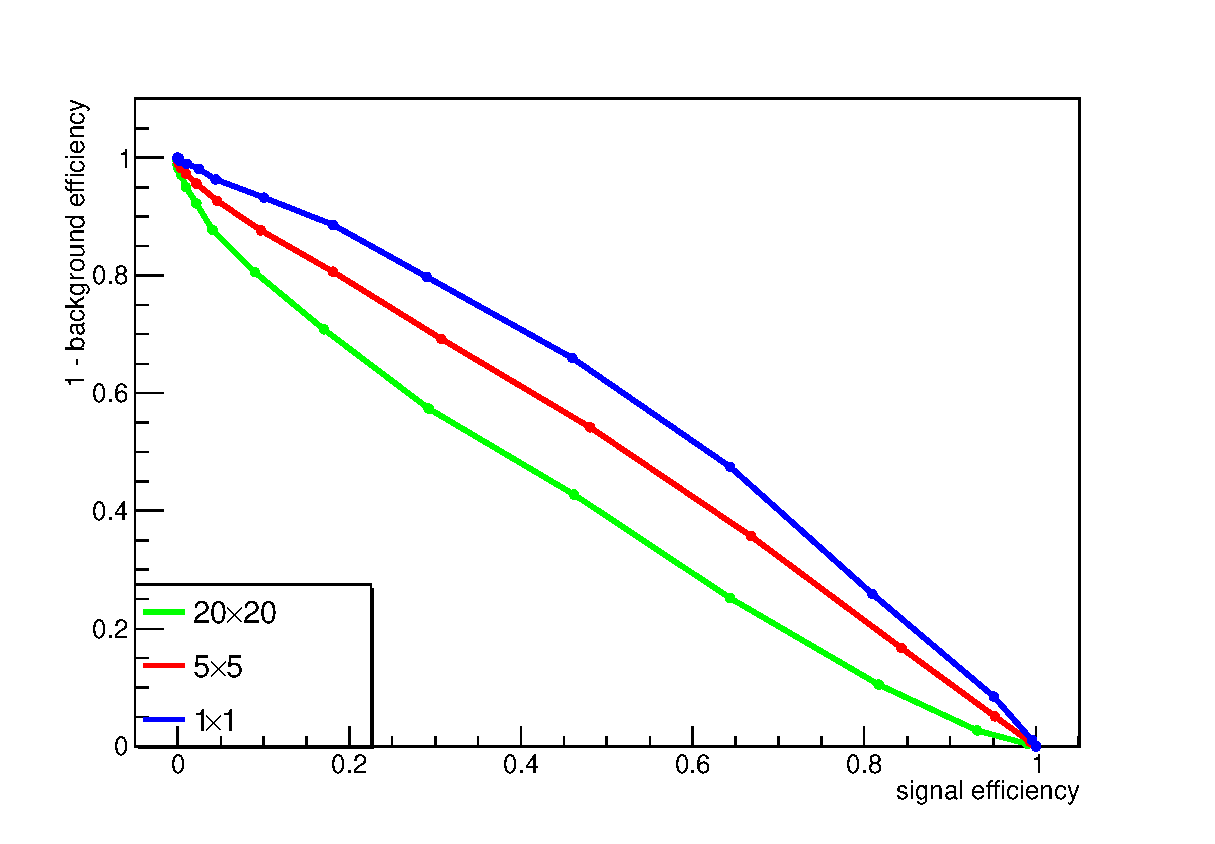
\includegraphics[width=0.43\textwidth]{figs/cluster_tau32_10_tev_eff.eps}
   }
   \subfigure[20 TeV] {
   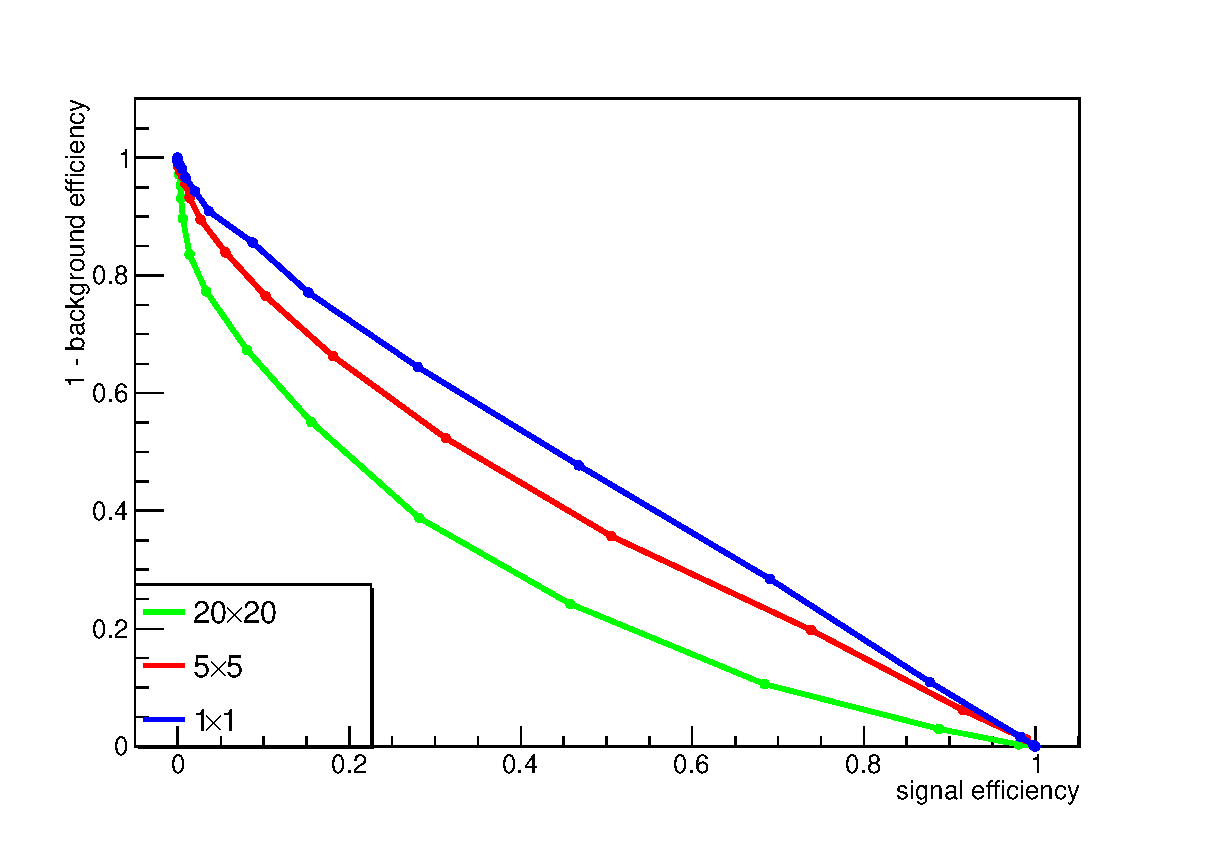
\includegraphics[width=0.43\textwidth]{figs/cluster_tau32_20_tev_eff.eps}
   }
   \subfigure[40 TeV] {
   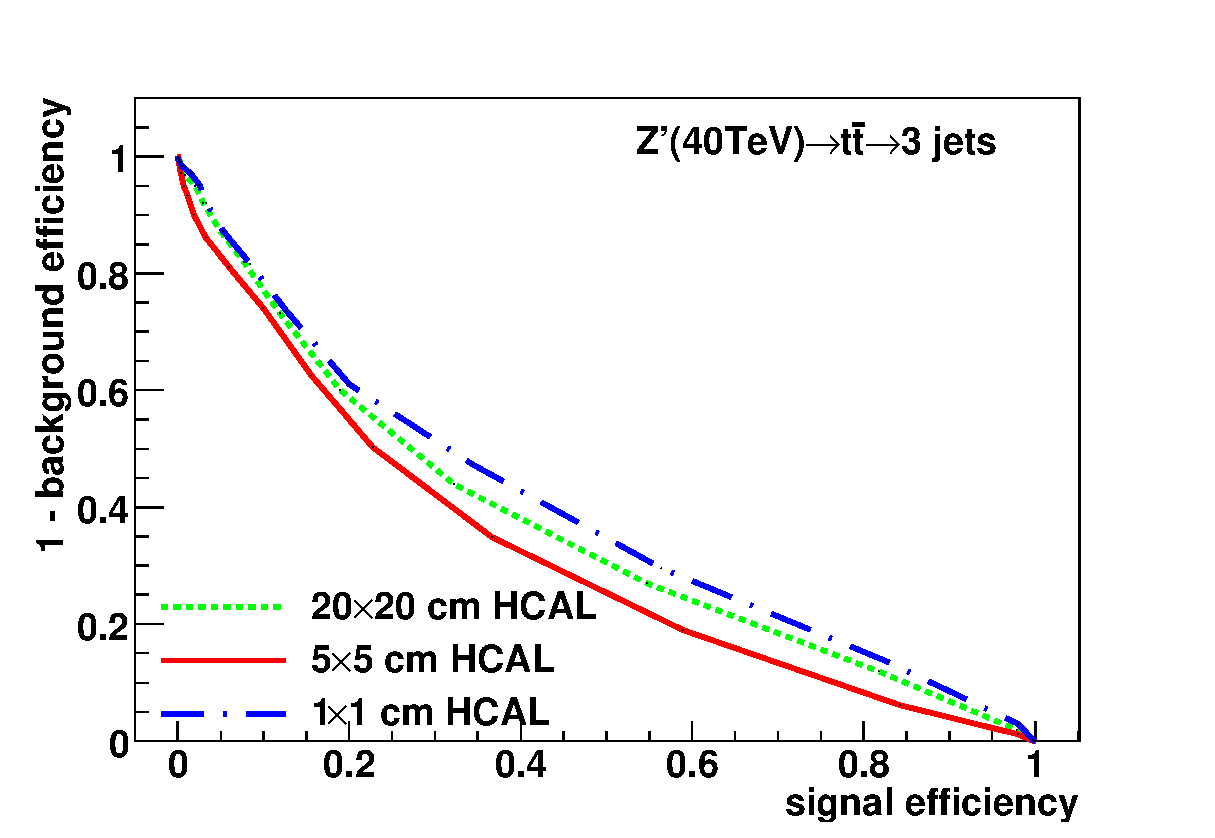
\includegraphics[width=0.43\textwidth]{figs/cluster_tau32_40_tev_eff.eps}
   }
\end{center}
\caption{Signal efficiency versus background rejection rate using $\tau_{32}$.The energies of collision at (a)5, (b)10, (c)20, (d)40TeV are shown here. In each picture, the three ROC curves correspond to different detector sizes.}
\label{fig:cluster_tau32}
\end{figure}

